\documentclass[conference]{IEEEtran}

\usepackage[utf8]{inputenc}
\usepackage{cite}
\usepackage{amsmath,amssymb,amsfonts}
\usepackage{graphicx}
\usepackage{xcolor}
\usepackage{tikz}
\usetikzlibrary{shapes.geometric, arrows.meta, positioning, fit, calc, backgrounds, patterns, circuits.logic.US, shapes.misc}
\usepackage{pgfplots}
\pgfplotsset{compat=1.17}
\usepackage{subcaption}
\usepackage{booktabs}

% Hardware component styles - PROPERLY SIZED
\tikzset{
    register/.style={
        rectangle,
        draw=black,
        thick,
        minimum width=1cm,
        minimum height=0.7cm,
        fill=white,
        font=\tiny\ttfamily
    },
    mux/.style={
        trapezium,
        trapezium left angle=70,
        trapezium right angle=110,
        draw=black,
        thick,
        minimum width=0.7cm,
        minimum height=0.6cm,
        fill=white,
        font=\tiny
    },
    alu/.style={
        rectangle,
        draw=black,
        thick,
        minimum width=0.9cm,
        minimum height=0.8cm,
        fill=white,
        font=\tiny
    },
    memory/.style={
        rectangle,
        draw=black,
        very thick,
        minimum width=0.9cm,
        minimum height=1cm,
        fill=white,
        font=\tiny
    },
    wire/.style={
        draw=black,
        thick,
        -Stealth
    },
    bus/.style={
        draw=black,
        line width=1.2pt,
        -Stealth
    },
    controlwire/.style={
        draw=black,
        dashed,
        -Stealth
    },
    buswidth/.style={
        font=\tiny,
        fill=white,
        inner sep=0.5pt
    },
    logic/.style={
        rectangle,
        draw=black,
        thick,
        rounded corners=2pt,
        minimum width=0.7cm,
        minimum height=0.6cm,
        fill=gray!10,
        font=\tiny
    },
    sbox/.style={
        rectangle,
        draw=black,
        thick,
        minimum width=0.55cm,
        minimum height=0.55cm,
        fill=gray!20,
        font=\tiny
    }
}

\begin{document}

\title{AES-128 Hardware Architecture:\\RTL Implementation on FPGA}

\author{\IEEEauthorblockN{Hardware Implementation}
\IEEEauthorblockA{Register-Transfer Level Design}}

\maketitle

%==============================================================================
% Figure 1: Complete Datapath - FIXED ARROWS
%==============================================================================
\begin{figure*}[!t]
\centering
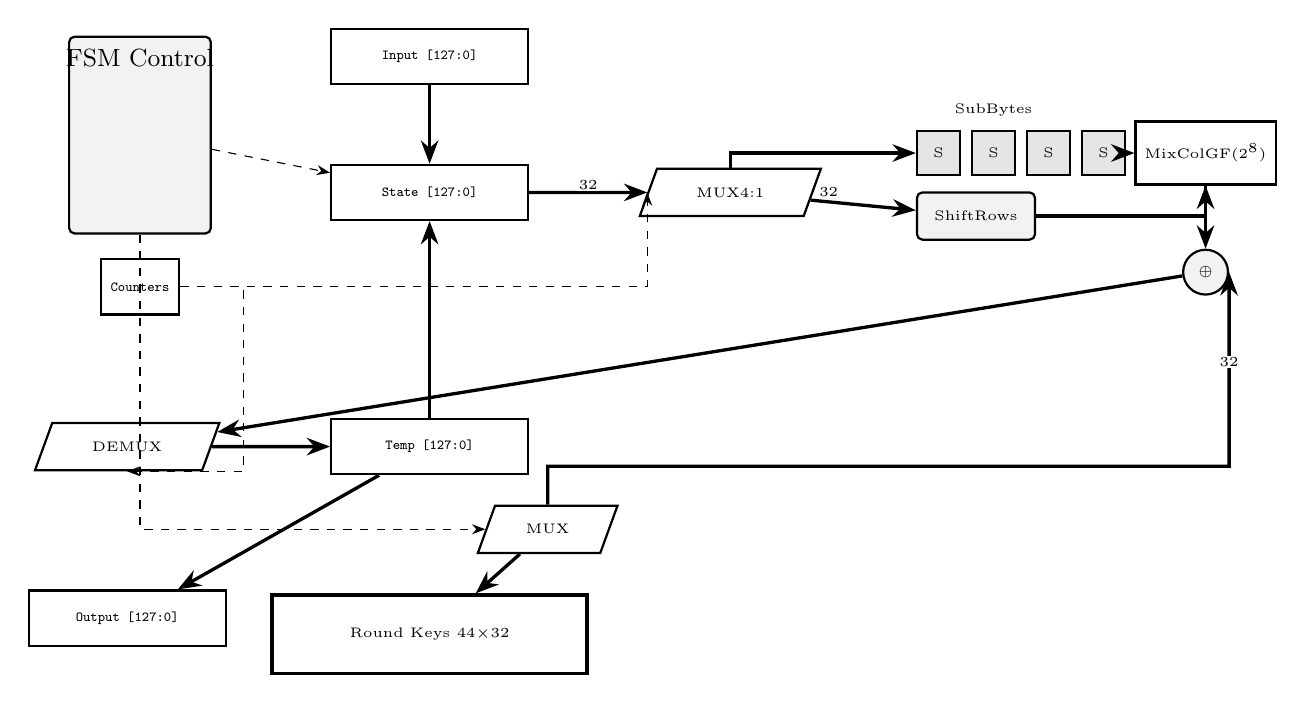
\begin{tikzpicture}[node distance=0.7cm and 1cm]

% Left side - Control and State
\node[logic, minimum width=1.8cm, minimum height=2.5cm] (fsm) at (0,0) {};
\node[font=\small, below=0.05cm of fsm.north] {FSM Control};

\node[register, minimum width=1cm, below=0.3cm of fsm] (counters) {Counters};

\node[register, minimum width=2.5cm, right=1.5cm of fsm, yshift=1cm] (input_reg) {Input [127:0]};
\node[register, minimum width=2.5cm, below=1cm of input_reg] (state_reg) {State [127:0]};
\node[register, minimum width=2.5cm, below=2.5cm of state_reg] (temp_reg) {Temp [127:0]};

% Middle - Datapath
\node[mux, right=1.5cm of state_reg, minimum width=1cm] (col_mux) {MUX\\4:1};
\node[buswidth, right=0.05cm of col_mux] {32};

\node[sbox, right=1.3cm of col_mux, yshift=0.5cm] (sbox0) {S};
\node[sbox, right=0.12cm of sbox0] (sbox1) {S};
\node[sbox, right=0.12cm of sbox1] (sbox2) {S};
\node[sbox, right=0.12cm of sbox2] (sbox3) {S};
\node[font=\tiny, above=0.05cm of sbox1] {SubBytes};

\node[logic, right=1.3cm of col_mux, yshift=-0.3cm, minimum width=1.5cm] (shift) {ShiftRows};

\node[alu, right=1.5cm of sbox1, minimum width=1.3cm] (mixcol) {MixCol\\GF($2^8$)};

\node[logic, circle, minimum size=0.5cm, below=0.8cm of mixcol] (xor) {$\oplus$};

\node[mux, left=1.5cm of temp_reg, shape border rotate=180] (demux) {DEMUX};

% Right side - Key
\node[memory, below=1.5cm of temp_reg, minimum width=4cm, minimum height=1cm] (keys) {Round Keys 44$\times$32};
\node[mux, above=0.5cm of keys, xshift=1.5cm, minimum width=0.8cm] (key_mux) {MUX};

\node[register, minimum width=2.5cm, below=1.5cm of demux] (output_reg) {Output [127:0]};

% Connections - Data
\draw[bus] (input_reg) -- (state_reg);
\draw[bus] (state_reg) -- node[buswidth, above] {32} (col_mux);
\draw[bus] (col_mux.north) |- (sbox0.west);
\draw[bus] (sbox3) -- (mixcol);  % FIXED: Direct connection
\draw[bus] (col_mux) -- (shift);  % FIXED: Direct connection
\draw[bus] (shift.east) -| (mixcol.south);
\draw[bus] (mixcol) -- (xor);
\draw[bus] (xor) -- (demux);  % FIXED: Direct connection
\draw[bus] (demux) -- (temp_reg);
\draw[bus] (temp_reg.north) -- (state_reg.south);
\draw[bus] (temp_reg) -- (output_reg);  % Already straight

% Key path
\draw[bus] (key_mux) -- (keys);  % FIXED: Direct connection
\draw[bus] (key_mux) -- ++(0,0.8) -| node[buswidth, near end, above] {32} (xor.east);

% Control
\draw[controlwire] (fsm) -- (state_reg);
\draw[controlwire] (counters) -| (col_mux.west);
\draw[controlwire] (counters.east) -- ++(0.8,0) |- (demux.south);
\draw[controlwire] (fsm) |- (key_mux.west);

\end{tikzpicture}
\caption{Complete AES datapath with RTL-level components showing 32-bit column-wise processing architecture.}
\label{fig:datapath}
\end{figure*}

\clearpage

%==============================================================================
% Figure 2: Pipeline Comparison - TWO SEPARATE SUBFIGURES
%==============================================================================
\begin{figure*}[!t]
\centering
\begin{subfigure}[b]{\textwidth}
\centering
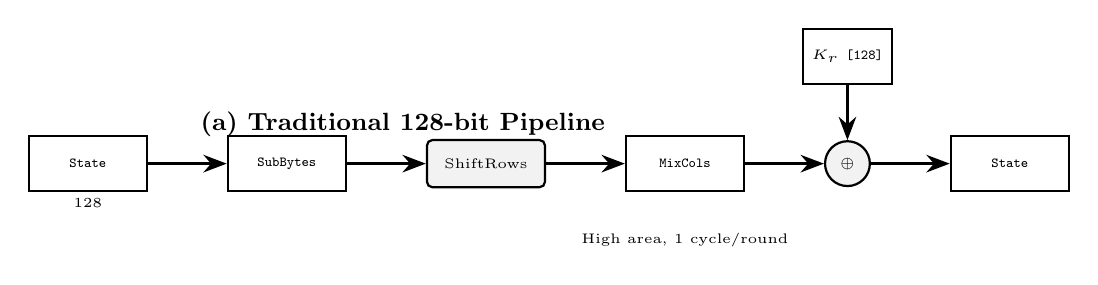
\begin{tikzpicture}[node distance=0.6cm and 1cm]

\node[font=\small\bfseries] at (4,0.5) {(a) Traditional 128-bit Pipeline};

\node[register, minimum width=1.5cm] (s0) at (0,0) {State};
\node[register, minimum width=1.5cm, right=of s0] (sb) {SubBytes};
\node[logic, right=of sb, minimum width=1.5cm] (sr) {ShiftRows};
\node[register, minimum width=1.5cm, right=of sr] (mc) {MixCols};
\node[logic, circle, minimum size=0.5cm, right=of mc] (xor) {$\oplus$};
\node[register, minimum width=1.5cm, right=of xor] (s1) {State};

\node[register, above=0.7cm of xor] (rk) {$K_r$ [128]};

\draw[bus] (s0) -- (sb);
\draw[bus] (sb) -- (sr);
\draw[bus] (sr) -- (mc);
\draw[bus] (mc) -- (xor);
\draw[bus] (xor) -- (s1);
\draw[bus] (rk) -- (xor);

\node[buswidth, below=0.05cm of s0.south] {128};
\node[font=\tiny, below=0.4cm of mc] {High area, 1 cycle/round};

\end{tikzpicture}
\end{subfigure}

\vspace{1cm}

\begin{subfigure}[b]{\textwidth}
\centering
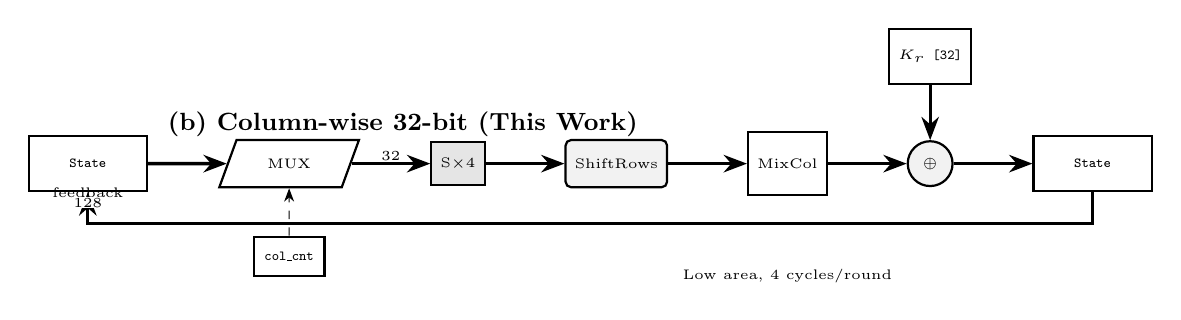
\begin{tikzpicture}[node distance=0.6cm and 1cm]

\node[font=\small\bfseries] at (4,0.5) {(b) Column-wise 32-bit (This Work)};

\node[register, minimum width=1.5cm] (s0) at (0,0) {State};
\node[mux, right=of s0] (mux) {MUX};
\node[sbox, right=of mux] (sb) {S$\times$4};
\node[logic, right=of sb, minimum width=1.2cm] (sr) {ShiftRows};
\node[alu, right=of sr, minimum width=1cm] (mc) {MixCol};
\node[logic, circle, minimum size=0.4cm, right=of mc] (xor) {$\oplus$};
\node[register, minimum width=1.5cm, right=of xor] (s1) {State};

\node[register, above=0.7cm of xor] (rk) {$K_r$ [32]};
\node[register, below=0.6cm of mux, minimum width=0.9cm, minimum height=0.5cm] (cnt) {col\_cnt};

\draw[bus] (s0) -- (mux);
\draw[bus] (mux) -- node[buswidth, above] {32} (sb);
\draw[bus] (sb) -- (sr);
\draw[bus] (sr) -- (mc);
\draw[bus] (mc) -- (xor);
\draw[bus] (xor) -- (s1);
\draw[bus] (rk) -- (xor);
\draw[bus] (s1.south) -- ++(0,-0.4) -| node[near end, above, font=\tiny] {feedback} (s0.south);
\draw[controlwire] (cnt) -- (mux);

\node[buswidth, below=0.05cm of s0.south] {128};
\node[font=\tiny, below=0.8cm of mc] {Low area, 4 cycles/round};

\end{tikzpicture}
\end{subfigure}

\caption{Pipeline comparison: (a) full-width vs (b) column-wise processing.}
\label{fig:pipeline}
\end{figure*}

\clearpage

%==============================================================================
% Figure 3: Key Expansion - CLEAN LAYOUT
%==============================================================================
\begin{figure}[!t]
\centering
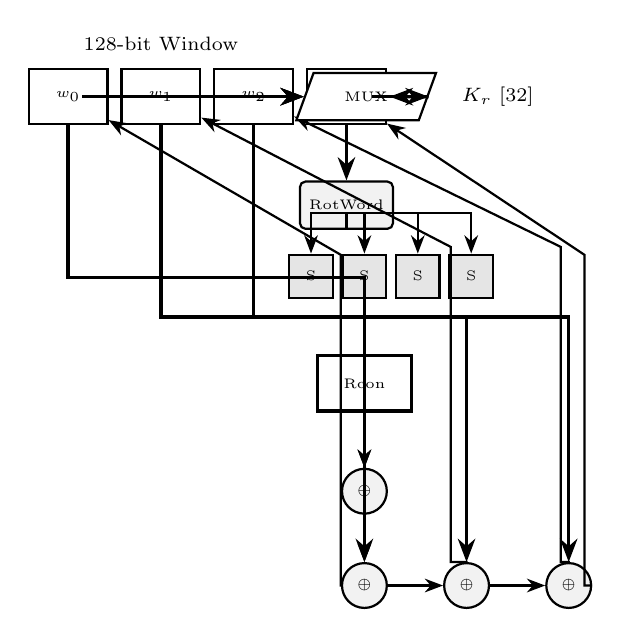
\begin{tikzpicture}[node distance=0.6cm and 0.7cm]

% Key registers
\node[register, minimum width=1cm] (w0) at (0,0) {$w_0$};
\node[register, minimum width=1cm, right=0.15cm of w0] (w1) {$w_1$};
\node[register, minimum width=1cm, right=0.15cm of w1] (w2) {$w_2$};
\node[register, minimum width=1cm, right=0.15cm of w2] (w3) {$w_3$};

\node[font=\scriptsize, above=0.1cm of w1] {128-bit Window};

% RotWord + SubWord
\node[logic, below=0.7cm of w3, minimum width=1cm] (rot) {RotWord};
\node[sbox, below=0.3cm of rot, xshift=-0.45cm] (s0) {S};
\node[sbox, right=0.1cm of s0] (s1) {S};
\node[sbox, right=0.1cm of s1] (s2) {S};
\node[sbox, right=0.1cm of s2] (s3) {S};

\draw[bus] (w3) -- (rot);
\draw[wire] (rot) -- ++(0,-0.1) -| (s0);
\draw[wire] (rot) -- ++(0,-0.1) -| (s1);
\draw[wire] (rot) -- ++(0,-0.1) -| (s2);
\draw[wire] (rot) -- ++(0,-0.1) -| (s3);

% Rcon + XOR
\node[memory, below=0.7cm of s1, minimum width=1.2cm, minimum height=0.7cm] (rcon) {Rcon};

\node[logic, circle, minimum size=0.4cm, below=0.7cm of rcon] (x1) {$\oplus$};
\node[logic, circle, minimum size=0.4cm, below=0.6cm of x1] (x2) {$\oplus$};
\node[logic, circle, minimum size=0.4cm, right=0.7cm of x2] (x3) {$\oplus$};
\node[logic, circle, minimum size=0.4cm, right=0.7cm of x3] (x4) {$\oplus$};

\draw[wire] (s1) -- ++(0,-0.2) -| (x1);
\draw[wire] (rcon) -- (x1);
\draw[bus] (w0) -- ++(0,-2.3) -| (x2);
\draw[wire] (x1) -- (x2);
\draw[wire] (x2) -- (x3);
\draw[bus] (w1) -- ++(0,-2.8) -| (x3);
\draw[bus] (w2) -- ++(0,-2.8) -| (x4);
\draw[wire] (x3) -- (x4);

% Feedback
\draw[wire] (x2) -- ++(-0.3,0) -- ++(0,4.2) -- (w0);
\draw[wire] (x3) -- ++(0,0.3) -- ++(-0.2,0) -- ++(0,4) -- (w1);
\draw[wire] (x4) -- ++(0,0.3) -- ++(-0.1,0) -- ++(0,4) -- (w2);
\draw[wire] (x4) -- ++(0.2,0) -- ++(0,4.2) -- (w3);

% Output
\node[mux, right=1.3cm of w1] (outmux) {MUX};
\draw[bus] (w0) -- ++(0.2,0) |- (outmux);
\draw[bus] (w1) -- ++(0.25,0) |- (outmux);
\draw[bus] (w2) -- ++(0.3,0) |- (outmux);
\draw[bus] (w3) -- ++(0.35,0) |- (outmux);
\node[right=0.3cm of outmux, font=\scriptsize] {$K_r$ [32]};
\draw[bus] (outmux) -- ++(0.3,0);

\end{tikzpicture}
\caption{On-the-fly key expansion with 4-word window (90\% memory reduction).}
\label{fig:keyexp}
\end{figure}

\clearpage

%==============================================================================
% Figure 4: SubBytes - VERTICAL LAYOUT
%==============================================================================
\begin{figure}[!t]
\centering
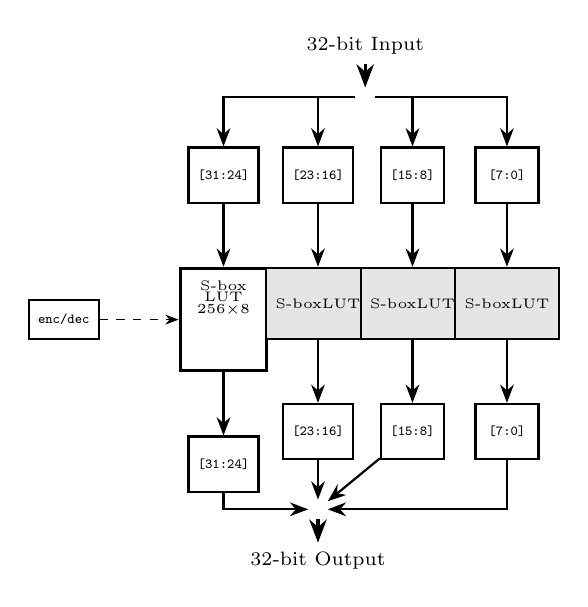
\begin{tikzpicture}[node distance=0.6cm]

\node[font=\scriptsize] (in) {32-bit Input};
\node[below=0.3cm of in] (split) {};

\node[register, below=0.5cm of split, xshift=-1.8cm, minimum width=0.8cm] (b0) {[31:24]};
\node[register, below=0.5cm of split, xshift=-0.6cm, minimum width=0.8cm] (b1) {[23:16]};
\node[register, below=0.5cm of split, xshift=0.6cm, minimum width=0.8cm] (b2) {[15:8]};
\node[register, below=0.5cm of split, xshift=1.8cm, minimum width=0.8cm] (b3) {[7:0]};

\draw[bus] (in) -- (split);
\draw[wire] (split) -| (b0);
\draw[wire] (split) -| (b1);
\draw[wire] (split) -| (b2);
\draw[wire] (split) -| (b3);

\node[memory, below=0.8cm of b0, minimum width=1.1cm, minimum height=1.3cm] (sb0) {};
\node[font=\tiny, below=0.05cm of sb0.north] {S-box};
\node[font=\tiny, below=0.2cm of sb0.north] {LUT};
\node[font=\tiny, below=0.35cm of sb0.north] {256$\times$8};

\node[sbox, below=0.8cm of b1, minimum width=0.9cm, minimum height=0.9cm] (sb1) {S-box\\LUT};
\node[sbox, below=0.8cm of b2, minimum width=0.9cm, minimum height=0.9cm] (sb2) {S-box\\LUT};
\node[sbox, below=0.8cm of b3, minimum width=0.9cm, minimum height=0.9cm] (sb3) {S-box\\LUT};

\draw[wire] (b0) -- (sb0);
\draw[wire] (b1) -- (sb1);
\draw[wire] (b2) -- (sb2);
\draw[wire] (b3) -- (sb3);

\node[register, below=0.8cm of sb0, minimum width=0.8cm] (o0) {[31:24]};
\node[register, below=0.8cm of sb1, minimum width=0.8cm] (o1) {[23:16]};
\node[register, below=0.8cm of sb2, minimum width=0.8cm] (o2) {[15:8]};
\node[register, below=0.8cm of sb3, minimum width=0.8cm] (o3) {[7:0]};

\draw[wire] (sb0) -- (o0);
\draw[wire] (sb1) -- (o1);
\draw[wire] (sb2) -- (o2);
\draw[wire] (sb3) -- (o3);

\node[below=0.5cm of o1] (merge) {};
\node[font=\scriptsize, below=0.3cm of merge] (out) {32-bit Output};

\draw[wire] (o0) |- (merge);
\draw[wire] (o1) -- (merge);
\draw[wire] (o2) -- (merge);
\draw[wire] (o3) |- (merge);
\draw[bus] (merge) -- (out);

\node[register, left=1cm of sb0, minimum width=0.8cm, minimum height=0.5cm] (mode) {enc/dec};
\draw[controlwire] (mode) -- (sb0);

\end{tikzpicture}
\caption{SubBytes with four parallel 256$\times$8 S-box LUTs for 32-bit processing.}
\label{fig:subbytes}
\end{figure}

\clearpage

%==============================================================================
% Figure 5: MixColumns - SIMPLIFIED
%==============================================================================
\begin{figure}[!t]
\centering
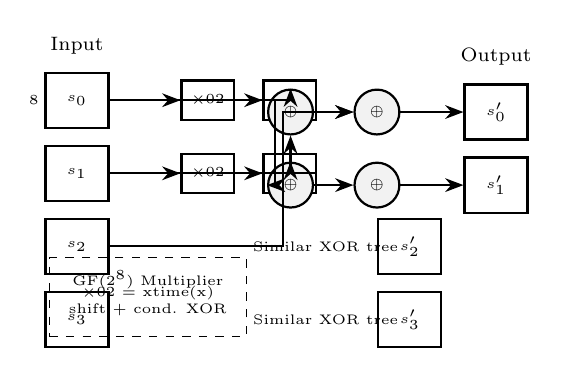
\begin{tikzpicture}[node distance=0.5cm and 0.6cm]

% Inputs
\node[register, minimum width=0.8cm] (s0) {$s_0$};
\node[register, minimum width=0.8cm, below=0.2cm of s0] (s1) {$s_1$};
\node[register, minimum width=0.8cm, below=0.2cm of s1] (s2) {$s_2$};
\node[register, minimum width=0.8cm, below=0.2cm of s2] (s3) {$s_3$};

\node[font=\scriptsize, above=0.1cm of s0] {Input};
\node[buswidth, left=0.05cm of s0] {8};

% GF mults (show for first two rows only)
\node[alu, right=0.9cm of s0, minimum width=0.65cm, minimum height=0.5cm] (m02_0) {$\times$02};
\node[alu, right=0.35cm of m02_0, minimum width=0.65cm, minimum height=0.5cm] (m03_0) {$\times$03};

\node[alu, right=0.9cm of s1, minimum width=0.65cm, minimum height=0.5cm] (m02_1) {$\times$02};
\node[alu, right=0.35cm of m02_1, minimum width=0.65cm, minimum height=0.5cm] (m03_1) {$\times$03};

\draw[wire] (s0) -- (m02_0);
\draw[wire] (s0.east) -- ++(0.3,0) |- (m03_0);
\draw[wire] (s1) -- (m02_1);
\draw[wire] (s1.east) -- ++(0.3,0) |- (m03_1);

% XOR trees
\node[logic, circle, minimum size=0.35cm, right=2cm of s0, yshift=-0.15cm] (x0) {$\oplus$};
\node[logic, circle, minimum size=0.35cm, right=0.5cm of x0] (x0b) {$\oplus$};

\node[logic, circle, minimum size=0.35cm, right=2cm of s1, yshift=-0.15cm] (x1) {$\oplus$};
\node[logic, circle, minimum size=0.35cm, right=0.5cm of x1] (x1b) {$\oplus$};

\draw[wire] (m02_0) -| (x0);
\draw[wire] (m03_1) -| (x0);
\draw[wire] (x0) -- (x0b);
\draw[wire] (s2.east) -- ++(2.2,0) |- (x0b);

\draw[wire] (m02_1) -| (x1);
\draw[wire] (s0.east) -- ++(2.1,0) |- (x1);
\draw[wire] (x1) -- (x1b);

% Outputs
\node[register, right=0.8cm of x0b, minimum width=0.8cm] (o0) {$s_0'$};
\node[register, right=0.8cm of x1b, minimum width=0.8cm] (o1) {$s_1'$};
\node[register, right=3.4cm of s2, minimum width=0.8cm] (o2) {$s_2'$};
\node[register, right=3.4cm of s3, minimum width=0.8cm] (o3) {$s_3'$};

\draw[wire] (x0b) -- (o0);
\draw[wire] (x1b) -- (o1);

\node[font=\tiny, right=1.7cm of s2] {Similar XOR tree};
\node[font=\tiny, right=1.7cm of s3] {Similar XOR tree};

\node[font=\scriptsize, above=0.1cm of o0] {Output};

% Detail box
\node[draw, dashed, below=0.7cm of s1, minimum width=2.5cm, minimum height=1cm, xshift=0.9cm] (detail) {};
\node[font=\tiny, below=0.05cm of detail.north] {GF($2^8$) Multiplier};
\node[font=\tiny, below=0.25cm of detail.north, align=center] {$\times$02 = xtime(x)\\shift + cond. XOR};

\end{tikzpicture}
\caption{MixColumns with GF($2^8$) multipliers and XOR trees for one column.}
\label{fig:mixcol}
\end{figure}

\clearpage

%==============================================================================
% Figure 6: Control FSM - CLEAR LAYOUT
%==============================================================================
\begin{figure}[!t]
\centering
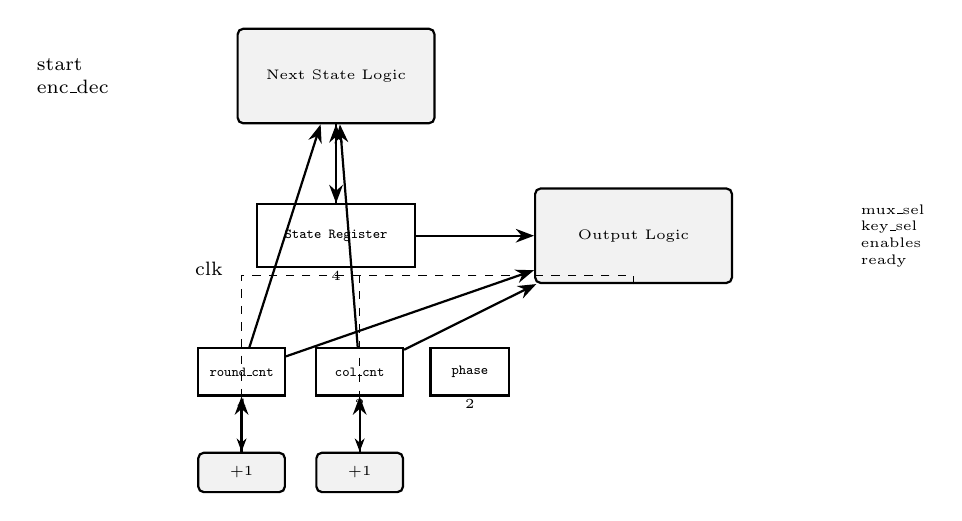
\begin{tikzpicture}[node distance=0.7cm and 1cm]

% State register
\node[register, minimum width=2cm, minimum height=0.8cm] (state) {State Register};
\node[buswidth, below=0.02cm of state.south] {4};

% Next state logic
\node[logic, above=1cm of state, minimum width=2.5cm, minimum height=1.2cm] (nsl) {Next State Logic};

% Output logic
\node[logic, right=1.5cm of state, minimum width=2.5cm, minimum height=1.2cm] (out) {Output Logic};

% Counters
\node[register, below=1cm of state, xshift=-1.2cm, minimum width=1.1cm, minimum height=0.6cm] (rc) {round\_cnt};
\node[buswidth, below=0.02cm of rc.south] {4};

\node[register, below=1cm of state, xshift=0.3cm, minimum width=1.1cm, minimum height=0.6cm] (cc) {col\_cnt};
\node[buswidth, below=0.02cm of cc.south] {2};

\node[register, below=1cm of state, xshift=1.7cm, minimum width=1cm, minimum height=0.6cm] (ph) {phase};
\node[buswidth, below=0.02cm of ph.south] {2};

% Increment
\node[logic, below=0.7cm of rc, minimum width=1.1cm, minimum height=0.5cm] (inc1) {+1};
\node[logic, below=0.7cm of cc, minimum width=1.1cm, minimum height=0.5cm] (inc2) {+1};

% Inputs/outputs
\node[left=1.5cm of nsl, font=\scriptsize, align=left] {start\\enc\_dec};
\node[right=1.5cm of out, font=\tiny, align=left] {mux\_sel\\key\_sel\\enables\\ready};

\draw[wire] (state) -- (nsl);
\draw[wire] (nsl) -- (state);
\draw[wire] (state) -- (out);

\draw[wire] (rc) -- (nsl);
\draw[wire] (cc) -- (nsl);
\draw[wire] (rc) -- (out);
\draw[wire] (cc) -- (out);

\draw[controlwire] (out) -- ++(0,-0.5) -| (inc1);
\draw[controlwire] (out) -- ++(0,-0.5) -| (inc2);
\draw[wire] (inc1) -- (rc);
\draw[wire] (inc2) -- (cc);

\node[font=\scriptsize, left=0.3cm of state.south west] {clk};

\end{tikzpicture}
\caption{Control FSM with state register, logic blocks, and counters.}
\label{fig:fsm}
\end{figure}

\end{document}
